\chapter{Proposed Method}
\section{System Architecture}
\begin{figure}[h]
\centering
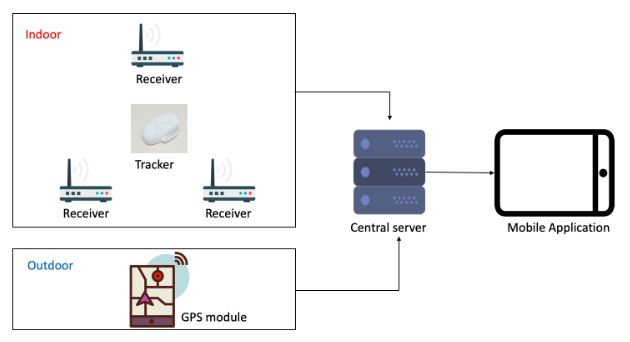
\includegraphics[width=\textwidth]{Image/System_Arch.JPG}
\caption{System Architecture}
\label{fig:system arch}
\end{figure}




\paragraph{}Our research plan to use system architecture shown in Figure~\ref{fig:system arch}. The system contains two main parts: indoor positioning and outdoor positioning. For indoor positioning, the system comprises of three main components: Tracker, Receiver, and Server. Tracker sends Bluetooth signal to the receiver. Then the receiver reads RSSI (Received Signal Strength Indicator) from received signal and sends it to the server. Afterwards, the server preprocesses the RSSI data and then calculate the position of the tracker. The preprocessing techniques used in our research are moving average and channel separation by K-means clustering method. After the data is preprocessed, it is fed into the path loss model in order to obtain the distance between the tracker and the receiver. Lastly, the trilateration method is used to acquire the position of the tracker. The tracker and receiver that we use is BLE (Bluetooth Low Energy) device and Raspberry Pi 3 respectively. The BLE device is used to transmit the Bluetooth signal at the sampling rate of 10 Hertz. The Raspberry Pi 3 is used for receiving the Bluetooth signal from the BLE device in form of RSSI (Received Signal Strength Indication) in decibel unit. Figure~\ref{fig:system arch} shows the devices that we use to collect the RSSI data. For outdoor positioning, the GPS (Global Positioning System) in mobile phone will be enabled when the tracker is no longer in the building, i.e. when the receiver does not receive any signal from the tracker. Figure~\ref{fig:component}a and ~\ref{fig:component}b depict the  device that we use to receiver The RSSI data and Tracker which send the RSSI data respectively  

\begin{figure}[h!]
\centering
\begin{subfigure}[b]{0.4\linewidth}
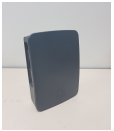
\includegraphics[width=\linewidth]{Image/rasp.png}
\caption{Receiver(RaspberryPi).}
\end{subfigure}
\begin{subfigure}[b]{0.4\linewidth}
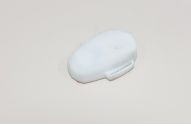
\includegraphics[width=\linewidth]{Image/tracker.png}
\caption{Tracker(Air-Node).}
\end{subfigure}
\caption{Component Deivices.}
\label{fig:component}
\end{figure}


\section{Software Architecture}

\paragraph{}Our software architecture comprises of four components: mobile application for displaying the target object position in 2D map, a cloud-host NoSql database for storing the position of the target object, server for calculating the position of target object, and GPS application for outdoor positioning that will be enabled when the target object is outside of the
building. The server and GPS application send the coordination data to NoSql database. Then the mobile application retrieves that data from database and renders it on 2D map. 
\section{System Process}
\begin{figure}[h]
\centering
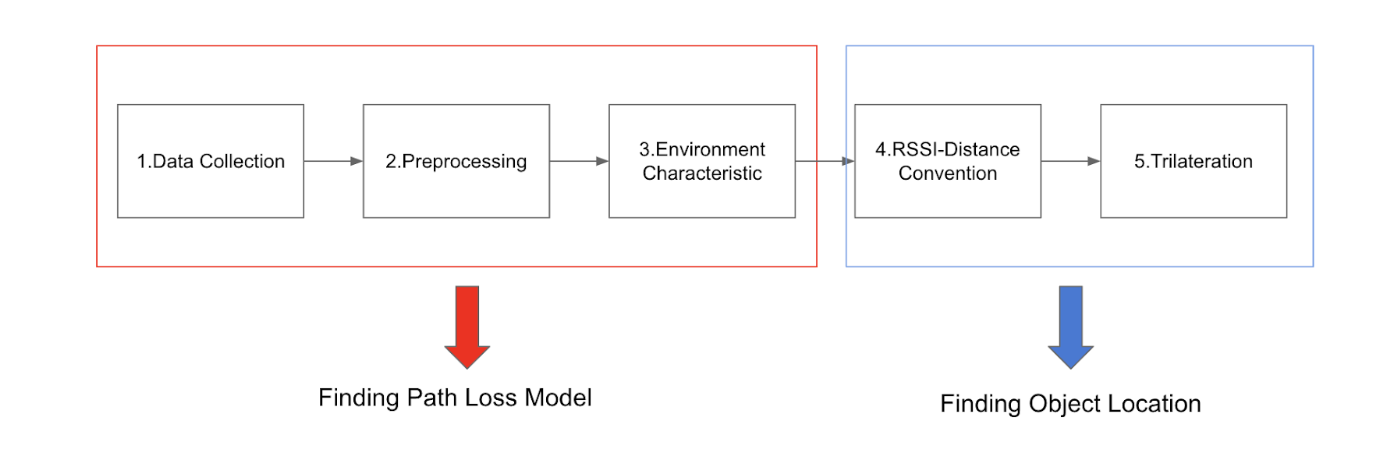
\includegraphics[width=\textwidth]{Image/systemprocess.png}
\label{system_topo}
\caption{System topology}
\end{figure}

\subsection{Data Collection}
\paragraph{}The first process of this section is data collection. In our system, the tracker
attached to the target object send out the Bluetooth signal (BLE). Then the receivers receive the signal from tracker, extract the RSSI data from it, and send that data to the server for further calculation. In the data collection process, the receiver and the tracker are placed on stands with a height of 1 meter. The receiver is placed on a fixed location while the BLE tracker is placed at different distances away from the receiver. At each distance, the tracker is rotated in eight different angles of rotation: 0, 45, 90, 135, 180, 225, 270 and 315 degrees.

\subsection{Preprocess}
\paragraph{}After collecting the raw RSSI data from data collection process, data preprocessing techniques are used for removing unnecessary data and smoothing the noisy data. Two different data preprocessing techniques are applied on the RSSI data of a specific tracker orientation, namely, moving average and channel separation.
\subsubsection{Moving Average}
\paragraph{}Moving average or moving mean is a method to smooth out short-term fluctuations and highlight longer-term trends or cycles by creating series of averages of subset of the whole data set.

\begin{equation}
\centering
y^\prime_1 = \frac{y_1+y_2+y_3+...+y_(w+1)-1}{w}
\label{fig:eqt1}
\end{equation}

\begin{equation}
\centering
y^\prime_2 = \frac{y_2+y_3+y_4+...+y_(w+2)-1}{w} 
\label{fig:eqt1}
\end{equation}

\paragraph{}Where $y^\prime_n$ is the data in the filtered data set, $y_n$ is the data from the original
set and $w$ is the window size. Since we are including the overlapped data, $y_n$will also include the original data at $y_2...y_(w+1)$ - 1in the calculation even though $y_2...y_(w+1) - 1$ is already included in the calculation of Eq. 4.1. After the process is done we will get a filtered data set $y$ which has a significantly less standard deviation than the original data set $y$ .thus, having less noise.

\subsubsection{Chanel Separation}
\paragraph{}The BLE uses three of the 40 channels for broadcasting its advertising packets. The collected data is separated into three clusters for each advertising channel. K-means clustering is performed to distinguish which of the three channels the data belongs to. For each channel, moving average is applied to
smooth the series of data.

\subsection{Environmental Characterization}
\paragraph{}The objective of this method is to find the value of n that constructs a curve that has the lowest total sum of squared error (SSE) or curve fitting process in Eq 4.3, meaning the best fit to the series of data points. SSE measures the deviation between the expected data point and the predicted data point produced by the curve fitting method. After obtaining the result of n, and then use n to substitute in Eq. 4.3 for create Path-loss model.

\begin{equation}
RSSI_d = RSSI_d\textsubscript{0}-10n\log_{10}\frac{d}{d0}
\label{fig:eqt3}
\end{equation}

\paragraph{}In figure\ref{system_topo}, show the example of result after using curve fitting process. Eq. 4.3 forms a curve that best fits this particular set of data points when n is equal to 2.6902 the data is collected in a free space environment. The best fit curve represents the path loss model of the specific environment where the data is collected, the specific angle of the tracker and the specific preprocessing technique performed on the data.
\begin{figure}[h]
\centering
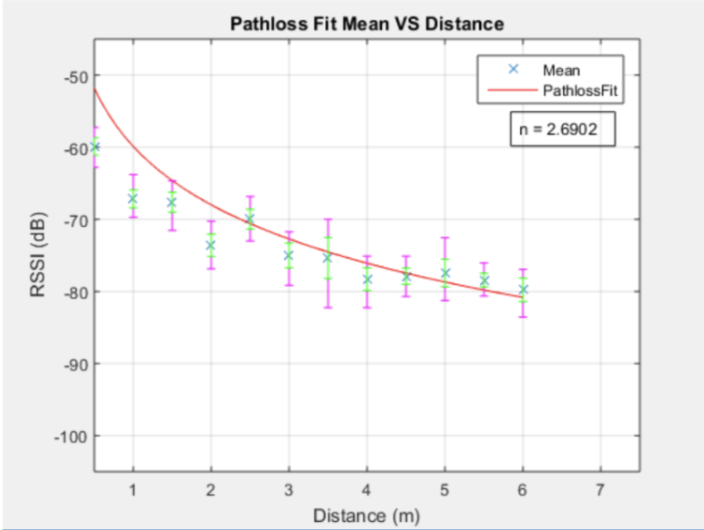
\includegraphics[width=\textwidth]{Image/angle0.png}
\caption{Angle 0, IC 6th floor}
\end{figure}

\newpage
\subsection{RSSI-Distance Conversion(Distance Estimation)}
\paragraph{}In this process, the RSSI value is collected continuously by at least three receivers. The collected RSSI data is preprocessed by the two preprocessing techniques and substituted into the corresponding path loss model to determine the distance between the target object and each receiver. The equation of the path loss model can be rearranged to solve for the distance as in Eq. (4.4).
\begin{equation}
d = d_010\frac{RSSI_d-RSSI_d\textsubscript{0}-X_\sigma}{-10n}
\label{fig:eqt4}
\end{equation}
\paragraph{}The $RSSId_0$ and $n$ is specific to each path loss model (determined in the previous process), while the $RSSI_d$ is obtained from either the mean or median of the preprocessed test set (e.g. mean of data preprocessed by moving average and channel separation, median of data preprocessed by moving median).
\subsection{Trilateration}
\paragraph{}Once we obtain the distances between the target object and each reference node as seen in Figure \ref{fig:self_positioning}, trilateration method can be applied to determine the exact location of the target object. Referring to Figure \ref{fig:tri}, Eq. (4.5), Eq. (4.6) and Eq. (4.7) can be constructed according to the Euclidean distance formula.
\begin{equation}
d_1^2 = (x-x_1)^2+(y - y_1)^2
\end{equation}
\begin{equation}
d_2^2 = (x-x_2)^2+(y - y_3)^2
\end{equation}
\begin{equation}
d_3^2 = (x-x_3)^2+(y - y_3)^2
\end{equation}
\paragraph{}Simplifying the above equations through several mathematical operations produce the following Eq. (4.8) and Eq. (4.9), where Eq. (4.8) is used to find the x coordinate of the target object and Eq. (4.9) is for the y coordinate.
\begin{equation*}
A = -2x_1+ 2x_2
\end{equation*}
\begin{equation*}
B= -2y_1+ 2y_2
\end{equation*}
\begin{equation*}
C = d_1^2- d_1^2-x_1^2+x_2^2-y_1^2+y_2^2
\end{equation*}
\begin{equation*}
D = -2x_2+ 2x_3
\end{equation*}
\begin{equation*}
E = -2x_2+ 2x_3
\end{equation*}
\begin{equation*}
F = d_2^2- d_3^2-x_2^2+x_3^2-y_2^2+y_3^2
\end{equation*}
\begin{equation}
X = \frac{CE-FB}{EA-BD}
\end{equation}
\begin{equation}
X = \frac{CD-AF}{BD-AE}
\end{equation}
\paragraph{}Knowing the coordinates of the three reference nodes (i.e. (x1, y1), (x2, y2), (x3, y3)) and the distances between the target node and the reference nodes (i.e. d1, d2, d3), these known values can be substituted into the equation to obtain the x and y coordinate of the target node.


